\section{Environment and System Details}
\label{sec:environment-details}

\subsection{RPG System Comparison}
\label{sec:system-comparison}

We analyze Pokémon RPG AI systems through a five-dimensional categorical framework $\mathcal{S}(\mathcal{A}) = (S, T, M, F, \Phi)$, characterizing state representation, tools, memory architecture, feedback mechanisms, and fine-tuning approach. Table~\ref{tab:system-comparison} illustrates this decomposition for each system as it was initially popularized.\footnote{These systems are under active development and have since adopted features---minimal additional information and self-reflection mechanisms---that were initially introduced by the \pokeagent project. We characterize each system at the version contemporaneous with PokeAgent's development (mid 2025), as later iterations increasingly converge on similar design choices (such as using sub-agents for feedback) without being completely open-source at the time of writing.} For current version capability for X Plays Pokémon, we encourage readers to directly view the stream of the individual creators. Many of these X Plays Pokémon baselines have completed numerous distinct Pokémon RPG games, which is very impressive from the view of the ML community. We recommend standardization among subsections of the game for easier comparison with state standardized by PokéAgent. For X Plays Pokémon, systems vary dramatically across each dimension: state representations range from visual frames to structured RAM extraction; tool availability ranges from basic button inputs to full planning suites with code execution; memory architectures span raw context windows to engineered summarization pipelines. Critically, even the reported evaluation metrics---variously ``steps,'' ``actions,'' and ``turns''---lack shared definitions across projects. These design choices dramatically affect measured performance, making cross-system comparison scientifically problematic without standardization.

\begin{table}[h]
\centering
\caption{Analysis of Pokémon RPG AI systems using the $(S, T, M, F, \Phi)$ framework, characterized at the version each system was initially popularized. Heterogeneity across dimensions makes direct performance comparison methodologically unsound without standardization.}
\label{tab:system-comparison}
\resizebox{\textwidth}{!}{%
\begin{tabular}{@{}lccccc@{}}
\toprule
\textbf{System} & \textbf{State $(S)$} & \textbf{Tools $(T)$} & \textbf{Memory $(M)$} & \textbf{Feedback $(F)$} & \textbf{Fine-tuning $(\Phi)$} \\
\midrule
Claude Plays Pokémon\textsuperscript{$\dagger$} & Frame + location, walkable tiles, party stats & Pathfinder, knowledge base & File-based summaries + knowledge base & ReAct loop & Zero-shot \\
GPT Plays Pokémon\textsuperscript{$\dagger$} & Frame + location, party stats, money, tile colors & Button inputs, self-built minimap & Goal tracker + notepad & Varied & Zero-shot \\
Gemini Plays Pokémon\textsuperscript{$\dagger$} & Frame + object positions, tile properties, navigability & Self-generated tools, code exec, pathfinder agent & Notepad + map markers + mental map & Varied & Zero-shot \\
Nunu AI & Frame + full parsed game state (map, party, items, NPCs) & Navigation, planning tools & Persistent memory store & ReAct loop + Twitch chat & Zero-shot \\
CLI Agents\textsuperscript{$\ddagger$} & Frame + map, party, bag & Game MCP tools (get state, press buttons, pathfinding) & Agent context window & ReAct loop & Zero-shot \\
\textbf{PokeAgent} & Frame + map, party, bag & Full MCP tool suite (pathfinding, memory, progress summary, reflection, etc)& knowledge base +  Action history window& Multi-agent self-reflection & Zero-shot \\
\bottomrule
\multicolumn{6}{l}{\textsuperscript{$\dagger$}Community-built harnesses, not official products of the respective model providers.} \\
\multicolumn{6}{l}{\textsuperscript{$\ddagger$}Claude Code, Codex CLI, Gemini CLI --- evaluated on the \pokeagent Speedrunning Track with standardized MCP tool access.} \\
\end{tabular}%
}
\end{table}

The key architectural distinction is in feedback and reflection. The ``X Plays Pokémon'' systems operate as observe-act loops: the model receives an observation, selects an action, and observes the result, with no explicit mechanism for evaluating its own decisions or recovering from errors. In contrast, \pokeagent employs a multi-agent self-reflection system in which a dedicated critic agent evaluates action outcomes, detects suboptimal play, and triggers strategy revision---enabling error recovery rather than error compounding. This distinction is not merely taxonomic: pure observe-act agents are known to exhibit ``panic behavior''~\citep{gemini2p5report}, where a single tactical mistake cascades into increasingly poor decisions, a failure mode that self-reflection explicitly mitigates.

A further distinction is in execution model. The ``X Plays Pokémon'' systems all freeze the emulator between actions, giving the model unlimited deliberation time per step---wall-clock runtimes of hundreds of hours are common (e.g., Gemini's 406-hour playthrough of Pokémon Blue). None penalize slow inference in their reported metrics, fully decoupling computational cost from any notion of real-time play. The \pokeagent Speedrunning Track, by contrast, measures wall-clock time as a primary metric: the emulator runs continuously and agents must issue actions in real time, penalizing slow inference and long reasoning chains. This makes speedrunning performance a joint measure of decision quality \emph{and} computational efficiency, more closely reflecting the practical constraints of deploying agents in interactive environments.


Among contemporary RPG systems, progress has been rapid but fragmented.
By early 2026, frontier models had completed full Pokémon playthroughs across multiple games---including Red, Blue, Crystal, and Emerald---using a variety of harness architectures.
Notable milestones include Gemini 2.5 Pro completing Pokémon Blue in approximately 406 hours~\citep{gemini2p5report,zhang2025geminiplayspokemon}, GPT-5 finishing Pokémon Red in 6,470 steps~\citep{engadget2025gptplayspokemon}, Gemini 3 Pro completing Pokémon Crystal~\citep{zhang2025gemini3playspokemon}, and later model iterations (GPT-5.1, GPT-5.2, Gemini 3 Flash) completing Crystal and Emerald as well.
Claude Plays Pokémon~\citep{anthropic2025visible} used chain-of-thought reasoning with a harness to complete a small section of the game over 35,000 actions, where its predecessor without these capabilities failed to exit the starting location.
However, these achievements resist direct comparison: the underlying harnesses differ fundamentally in state representation, tool access, and action granularity, and even the reported metrics---variously ``steps,'' ``actions,'' and ``turns''---lack shared definitions across projects.
The \pokeagent Challenge Speedrunning Track addresses precisely this gap, providing a standardized state and evaluation protocol that enables verified, apples-to-apples comparisons across models and harnesses.

See Appendix~\ref{sec:baseline-architectures} for detailed architecture descriptions of our baselines, including the \pokeagent multi-agent orchestration system.

\subsubsection{Speedrunning: Evaluation Interface}

\begin{figure}[H]
    \centering
    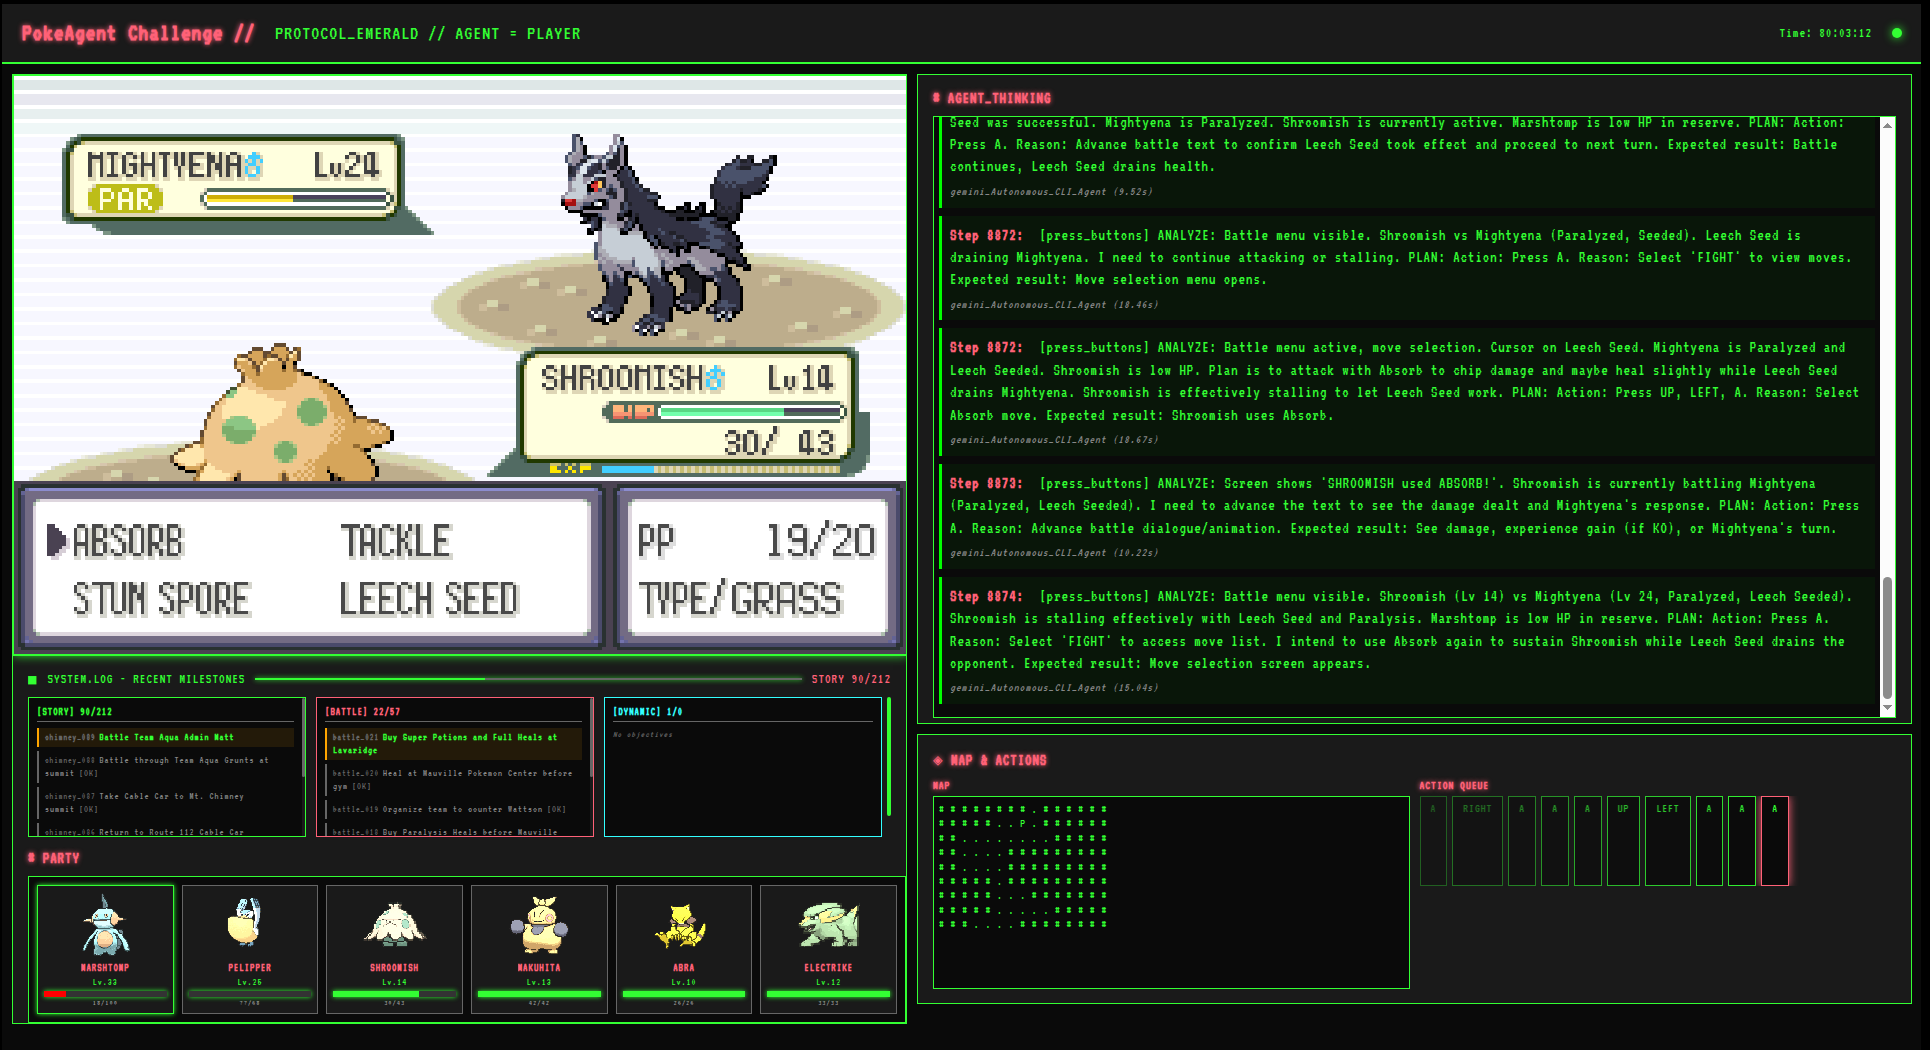
\includegraphics[width=\linewidth]{figures/layout.png}
    \caption{\textbf{Speedrunning Track Evaluation Interface.} The interface displays: (1) the Pokémon Emerald game screen showing a trainer battle with move selection (top left), (2) agent reasoning traces with timestamped decision logs detailing battle strategy and action rationale (right panel), (3) current party composition with sprite previews (bottom left), and (4) map overview with action history (bottom right). This visualization enables real-time debugging of agent behavior across the thousands of timesteps required for speedrunning.}
    \label{fig:track2_interface}
\end{figure}

\subsection{LLM Baseline Token Usage and Cost}
\label{sec:llm-cost}

Table~\ref{tab:llm-cost} reports token consumption and API cost for each LLM baseline on the Gen~9 OU Extended Timer ladder. Costs vary by over $70\times$ across models: GPT-5.2 is the most expensive at \$1.247 per game, while DeepSeek~V3 and Qwen3.5 Plus cost roughly \$0.015. Output token counts per turn also vary dramatically---MiniMax produces $\sim$6.2K completion tokens per turn, whereas DeepSeek~V3 and Qwen3.5 Plus produce fewer than 10. These differences highlight that raw per-game cost is driven primarily by output pricing and reasoning verbosity rather than game length.

\begin{table}[h]
\centering
\small
\caption{LLM baseline token usage and API cost on the Gen~9 OU Extended Timer ladder. Input/output tokens are per-turn averages. Models sorted by GXE rank (descending).}
\label{tab:llm-cost}
\resizebox{\textwidth}{!}{%
\begin{tabular}{@{}lrrrrrr@{}}
\toprule
\textbf{Model} & \textbf{Avg Input Tok/Turn} & \textbf{Avg Output Tok/Turn} & \textbf{Avg Turns} & \textbf{Avg Cost/Game} & \textbf{Avg Cost/Turn} & \textbf{Total Cost} \\
\midrule
Gemini 3.1 Pro    & 1,245 &     54 & 21.1 & \$0.066  & \$0.0031 &   \$8.86 \\
GPT-5.2           & 2,472 &  4,270 & 17.8 & \$1.247  & \$0.0702 & \$162.16 \\
Gemini 3 Flash    & 1,265 &     76 & 23.7 & \$0.020  & \$0.0009 &   \$0.90 \\
GLM-5             & 1,658 &    960 & 18.3 & \$0.069  & \$0.0038 &   \$7.98 \\
Gemini 3 Pro      & 1,211 &    115 & 23.9 & \$0.091  & \$0.0038 &   \$3.72 \\
Claude Opus 4.6   & 2,110 &    137 & 24.4 & \$0.341  & \$0.0140 &  \$73.59 \\
Grok-3 Mini       & 1,902 &  1,262 & 23.7 & \$0.029  & \$0.0012 &   \$4.27 \\
Claude Sonnet 4.6 & 2,234 &    132 & 23.7 & \$0.206  & \$0.0087 &  \$34.83 \\
Grok-3            & 1,971 &      9 & 22.2 & \$0.134  & \$0.0061 &  \$24.96 \\
MiniMax M2.5      & 2,327 &  6,218 & 18.3 & \$0.120  & \$0.0065 &   \$1.31 \\
Hermes 4 405B     & 2,310 &     91 & 21.7 & \$0.056  & \$0.0026 &   \$7.22 \\
DeepSeek V3       & 2,238 &      9 & 23.5 & \$0.017  & \$0.0007 &   \$3.42 \\
Kimi K2.5         & 1,900 &  4,510 & 19.2 & \$0.207  & \$0.0108 &   \$3.72 \\
Qwen3.5 Plus      & 2,306 &      8 & 22.9 & \$0.014  & \$0.0006 &   \$2.55 \\
\bottomrule
\end{tabular}%
}
\end{table}

\subsection{Speedrunning Track Task Diversity}

\begin{figure}[h]
    \centering
    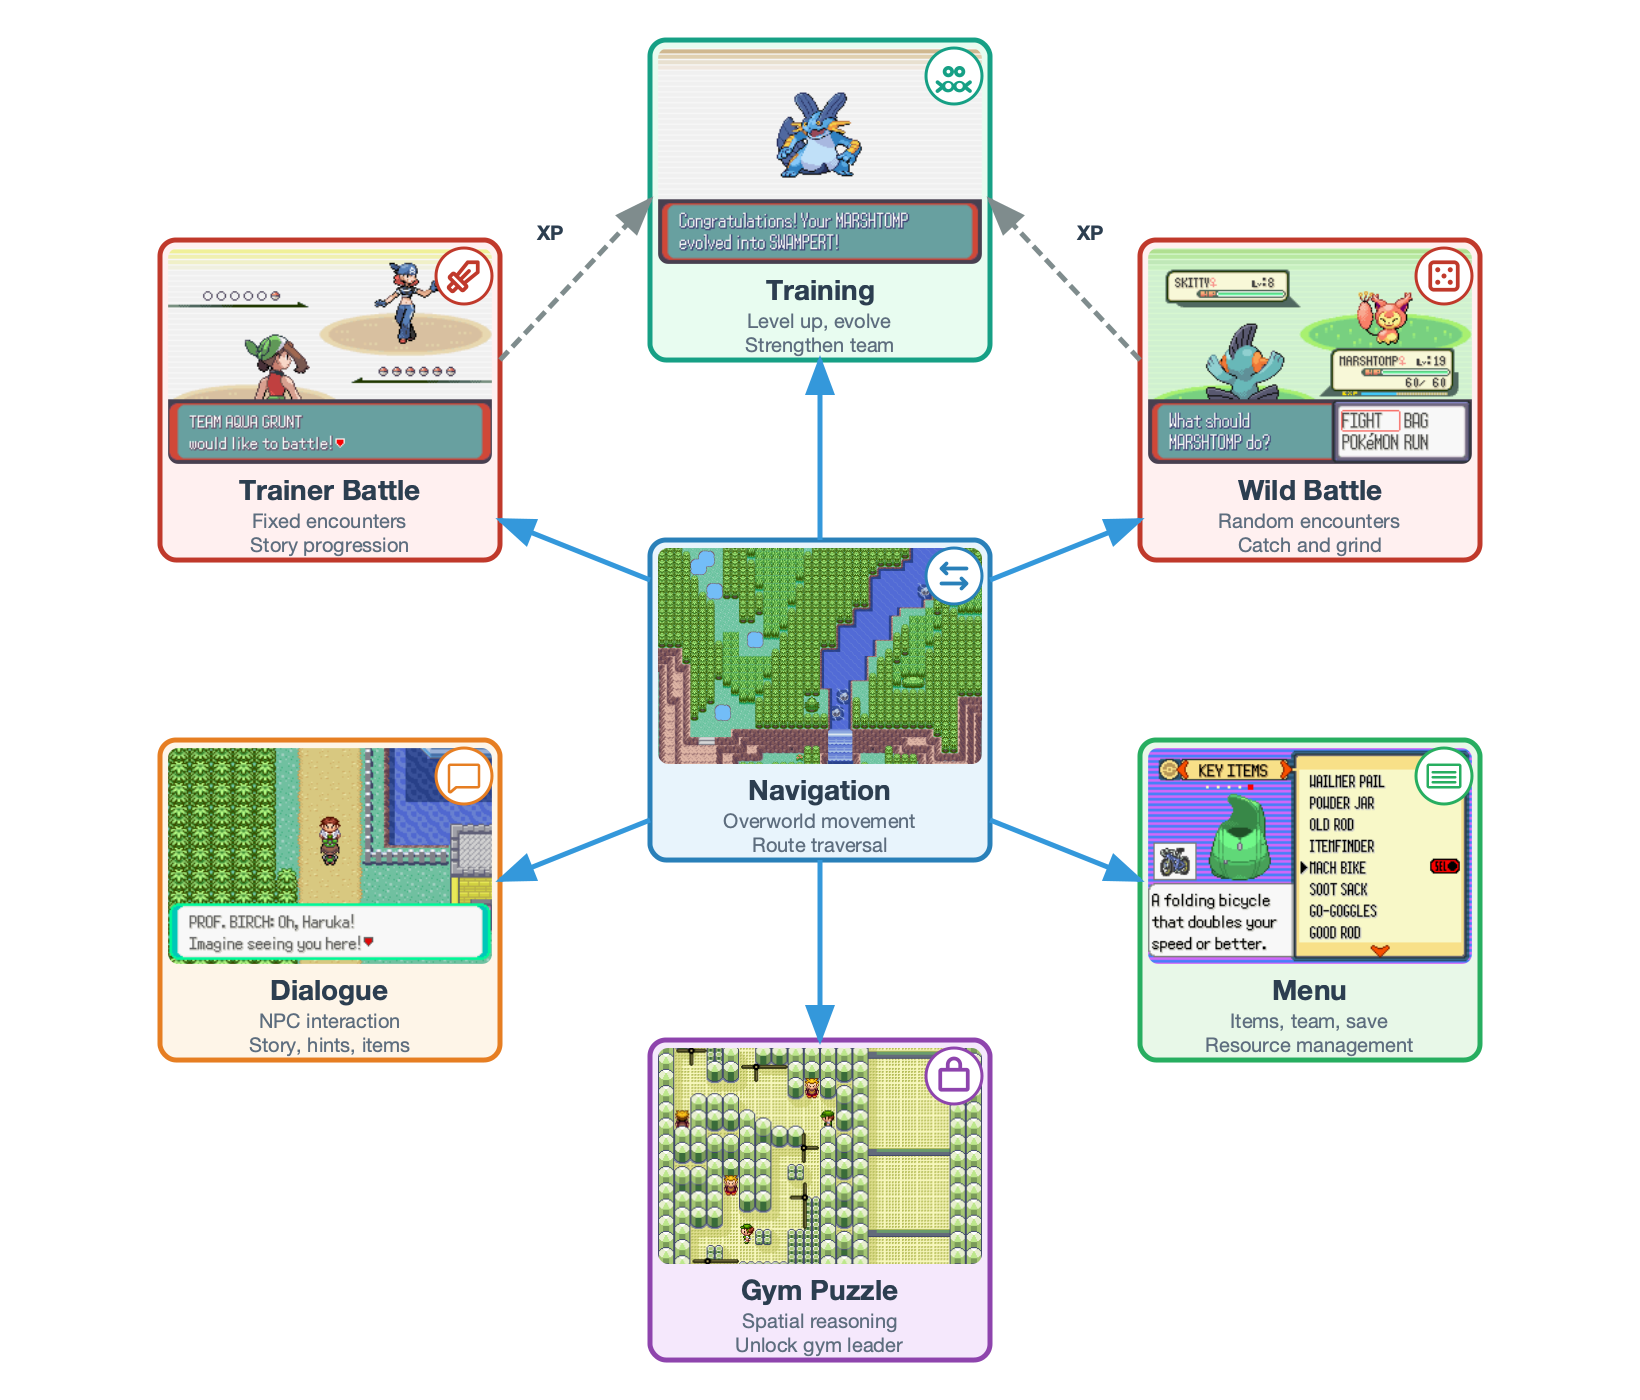
\includegraphics[width=\linewidth]{figures/track2_tasks.png}
    \caption{\textbf{Speedrunning Track Task Diversity.} Directed graph showing RPG subtask categories and their dependencies. Core tasks include overworld navigation, battle encounters (wild and trainer), gym puzzles, menu management, and NPC dialogue. Edges indicate how completing one task type enables or requires others---for example, navigation leads to encounters, battles yield experience for team building, and menu interactions manage resources needed for all other tasks.}
    \label{fig:track2_tasks}
\end{figure}

